\section{Vertiefungsprojekt: N-Damen Problem mittels Choco-Solver}

Um besser zu verstehen, wie Constraint-Probleme mit konventionellen Programmiersprachen gel�st werden, wurde das N-Queen-Problem in Java implementiert.

\begin{figure}[H]
    \centering
    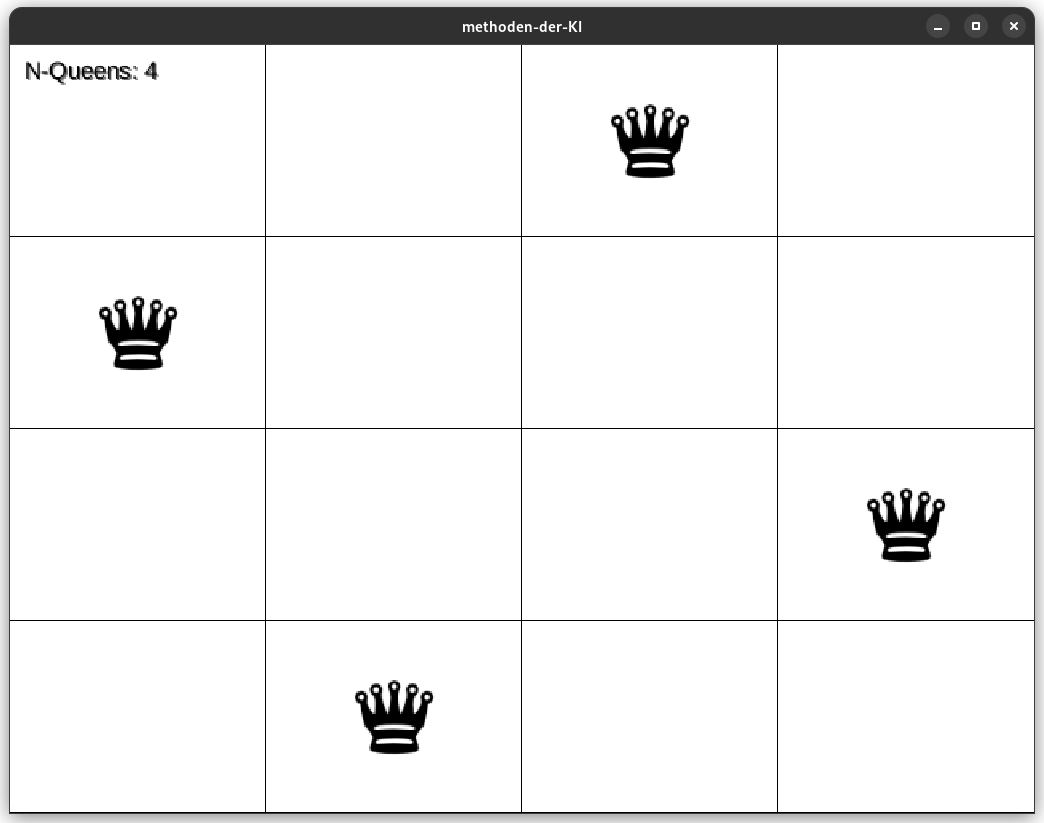
\includegraphics[width=0.8\textwidth]{figures/kap5/n-queens-impl.png}
    \caption{N-Damen Implementierung mit n=4}
    \label{fig:impl-n-damen}
\end{figure}

In diesem Programm wird das n-Damen-Problem f�r n=4 bis 27 unter Verwendung von Constraints gel�st. In diesem Programm w�rde das Dr�cken der Aufw�rts- und Abw�rtspfeiltasten den Wert von N entsprechend erh�hen oder verringern. Das Gitter aktualisiert sich dann selbst, um n x n beizubehalten, und der Choco-Cosntraintssl�ser wird jedes Mal verwendet, wenn sich n �ndert, um eine L�sung zu generieren. Das Programm funktioniert f�r Werte von n von 4 bis 27, aber da die Gr��e des Damenbildes nicht skaliert, ist es schwer zu sehen, wo genau eine Dame nach n=18 platziert wird.

Die Tastensteuerungen wie folgt:
\begin{itemize}
    \item \textbf{Up Arrow Key:} Erh�ht den Wert von N.
    \item \textbf{Down Arrow Key:} Verringert den Wert von N.
    \item \textbf{Escape-Taste:} Geht zur�ck zum Start-Screen.
\end{itemize}

Der relevante Code f�r das Programm befindet sich in den folgenden Packages:
\begin{itemize}
    \item \textbf{de.augsburg.hs.methoden.ki.algorithms.constraints:} Implementierung der Constraints mit Choco-Solver.
    \item \textbf{de.augsburg.hs.methoden.ki.screens.minmax} Klasse f�r den N-Queen-Screen.
    \item \textbf{de.augsburg.hs.methoden.ki.actors.nqueens:} Klassen f�r die Darstellung der Damen.
\end{itemize}